% !TeX root = RJwrapper.tex
\title{ToOoOlTiPs: An R package for Customizable Tooltips in Interactive
Graphics}
\author{by Quietest Quokka and Bounciest Bilby}

\maketitle

\abstract{%
An abstract of less than 150 words.
}

\hypertarget{introduction}{%
\section{Introduction}\label{introduction}}

Interactive graphics is a type of visualization that allows users to
interactively inspect a plot. One of the most basic interactivity is
through tooltips, where users can request additional information about a
plot element by mouse hovering \ldots{}

This paper will first review some R packages on interactive graphics and
their tooltip implementations. Next, a new package \CRANpkg{ToOoOlTiPs}
will be proposed for customizing tooltips. Some gallery plots will then
be given to showcase how these tooltips help users to better read the
graphics.

\hypertarget{literacture-review}{%
\section{Literacture review}\label{literacture-review}}

Some packages on interactive graphics include \CRANpkg{plotly}
\citep{plotly} that interfaces with Javascript for web-based interactive
graphics, \CRANpkg{crosstalk} \citep{crosstalk} that specializes
cross-linking elements across individual graphics, and most recently,
\CRANpkg{tsibbletalk} \citep{RJ-2021-050} for working with time series
data in a tsibble structure \ldots{}

\hypertarget{customizing-tooltip-design-with}{%
\section{\texorpdfstring{Customizing tooltip design with
\pkg{ToOoOlTiPs}}{Customizing tooltip design with }}\label{customizing-tooltip-design-with}}

\pkg{ToOoOlTiPs} is a packages for customizing tooltips in interactive
graphics, it features \ldots{}

\hypertarget{a-gallery-of-tooltips}{%
\section{A gallery of tooltips}\label{a-gallery-of-tooltips}}

We first show a baseline plot, in Figure \ref{fig:penguins-plotly}, made
by the \pkg{plotly} package with \CRANpkg{palmerpenguin} data
\citep{palmerpenguins}.

\begin{Schunk}
\begin{Sinput}
p <- penguins %>% 
  ggplot(aes(x = bill_depth_mm, y = bill_length_mm, 
             color = species)) + 
  geom_point()
ggplotly(p)
\end{Sinput}
\begin{figure}
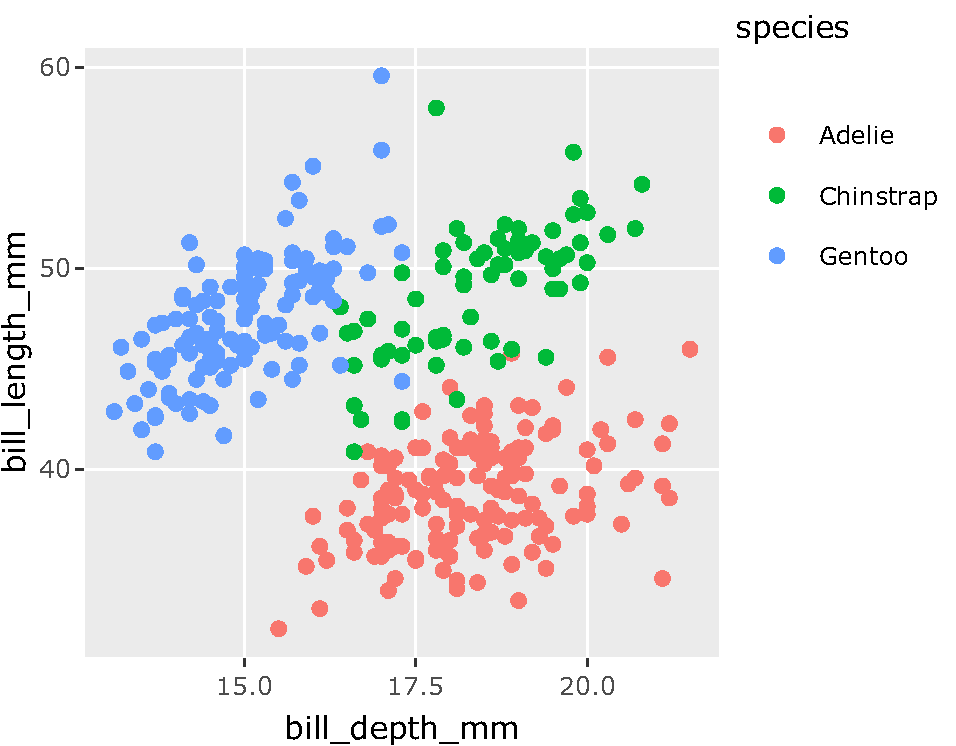
\includegraphics{sample-article_files/figure-latex/penguins-plotly-1} \caption[A basic interactive plot made with the plotly package on palmer penguin data]{A basic interactive plot made with the plotly package on palmer penguin data. Three species of penguins are plotted with bill depth on the x-axis and bill length on the y-axis. When hovering on a point, a tooltip will show the exact value of the bill depth and length for that point, along with the species name.}\label{fig:penguins-plotly}
\end{figure}
\end{Schunk}

Now we will re-create the same plot using the \pkg{ToOoOlTiPs} package
for different tooltips designs \ldots{}

\hypertarget{summary}{%
\section{Summary}\label{summary}}

We have displayed various tooltips that are available in the package
\pkg{ToOoOlTiPs}. These tooltips \ldots{}

\bibliography{sample-article.bib}

\address{%
Quietest Quokka\\
University of Little Mates\\%
Department of Letter Q\\ Somewhere, Australia\\
%
\url{https://www.britannica.com/animal/quokka}%
\\\textit{ORCiD: \href{https://orcid.org/0000-1721-1511-1101}{0000-1721-1511-1101}}%
\\\href{mailto:qquo@ulm.edu}{\nolinkurl{qquo@ulm.edu}}
}

\address{%
Bounciest Bilby\\
University of Little Mates\\%
Department of Letter B\\ Somewhere, Australia\\
%
\url{https://www.britannica.com/animal/bilby}%
\\\textit{ORCiD: \href{https://orcid.org/0000-0002-0912-0225}{0000-0002-0912-0225}}%
\\\href{mailto:bbil@ulm.edu}{\nolinkurl{bbil@ulm.edu}}
}
